\documentclass{beamer}
\usetheme{Boadilla}
\usepackage{xcolor}
\definecolor{olive}{rgb}{0.3, 0.4, .1}
\definecolor{fore}{RGB}{249,242,215}
\definecolor{back}{RGB}{51,51,51}
\definecolor{title}{RGB}{255,0,90}
\definecolor{dgreen}{rgb}{0.,0.6,0.}
\definecolor{gold}{rgb}{1.,0.84,0.}
\definecolor{JungleGreen}{cmyk}{0.99,0,0.52,0}
\definecolor{BlueGreen}{cmyk}{0.85,0,0.33,0}
\definecolor{RawSienna}{cmyk}{0,0.72,1,0.45}
\definecolor{Magenta}{cmyk}{0,1,0,0}
\newcommand{\blue}[1]{\textcolor{blue}{#1}}
\newcommand{\green}[1]{\textcolor{green}{#1}}
\newcommand{\dgreen}[1]{\textcolor{dgreen}{#1}}
\newcommand{\orange}[1]{\textcolor{orange}{#1}}
\newcommand{\red}[1]{\textcolor{red}{#1}}
\newcommand{\purple}[1]{\textcolor{purple}{#1}}
\newcommand{\olive}[1]{\textcolor{olive}{#1}}

\newcommand{\cL}{\mathcal{L}}
\newcommand{\cO}{\mathcal{O}}
\newcommand{\cR}{\mathcal{R}}

\newcommand{\bbC}{\mathbb{C}}
\newcommand{\bbQ}{\mathbb{Q}}
\newcommand{\bbR}{\mathbb{R}}
\newcommand{\bbZ}{\mathbb{Z}}

\newcommand{\Tr}{\mathrm{Tr}}
\newcommand{\TrKQ}{\mathrm{Tr}_{K/\mathbb{Q}}}
\newcommand{\TrKRR}{\mathrm{Tr}_{K_{\mathbb{R}}/\mathbb{R}}}
\newcommand{\TrKRpR}{\mathrm{Tr}_{K_{\mathbb{R}'}/\mathbb{R}}}
\newcommand{\NKQ}{\mathrm{N}_{K/\mathbb{Q}}}
\newcommand{\cOL}{\mathcal{O}^{\mathcal{L}}}
\newcommand{\cOV}{\mathcal{O}^{\vee}}
\newcommand{\cOLp}{\mathcal{O}^{\mathcal{L'}}}
\newcommand{\cLV}{\mathcal{L}^{\vee}}
\newcommand{\cLpV}{(\mathcal{L'})^{\vee}}
\newcommand{\cOpV}{(\mathcal{O'})^{\vee}}
\newcommand{\KR}{K_{\mathbb{R}}}
\newcommand{\va}{\vec{a}}
\newcommand{\vb}{\vec{b}}
\newcommand{\vc}{\vec{c}}
\newcommand{\ve}{\vec{e}}
\newcommand{\vp}{\vec{p}}
\newcommand{\vr}{\vec{r}}
\newcommand{\vs}{\vec{s}}
\newcommand{\vx}{\vec{x}}
\newcommand{\vy}{\vec{y}}
\newcommand{\vbV}{\vec{b}^{\vee}}
\newcommand{\vcV}{\vec{c}^{\vee}}
\newcommand{\vpV}{\vec{p}^{\vee}}

\newcommand{\divline}{\noindent\rule{6cm}{0.4pt}}
% \usepackage{beamerthemesplit} // Activate for custom appearance

\title{Algebraically Structured LWE, Revisited}
\subtitle{Chris Peikert, Zachary Pepin}
\author{Yuncong Zhang}
\date{May 22, 2020}

\begin{document}

\frame{\titlepage}

\frame{\frametitle{Outline}\tableofcontents}

\section{Introduction}
\frame
{
  \frametitle{Background}
  Regev proposed the \blue{original LWE} [Reg09]

  \begin{itemize}
  	\item Average-case to worst-case security
  	\item Impractical efficiency
  \end{itemize}

  \blue{Structured LWE}s are LWEs with special structure on matrix $A$
  \begin{figure}[ht!]
  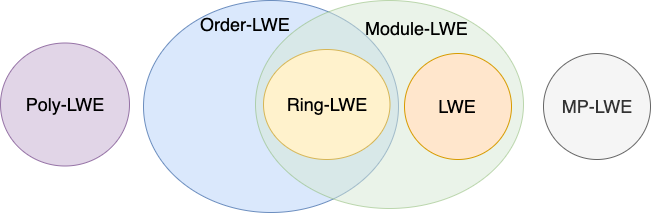
\includegraphics[width=0.5\textwidth]{files/Structured-LWE.png}
  \end{figure}

  \dgreen{Advantage: improved efficiency}\\
  \red{Disadvantages: complex security reduction}

}

\frame
{
  \frametitle{Contribution of this Paper}
  \begin{itemize}
  	\item A \blue{framework} that encompasses \orange{ALL} structured LWEs

  	\item A \blue{new LWE} that \orange{generalizes} algebraic LWEs

  	\item Use the framework to give much \dgreen{simpler}, \dgreen{more general}, and \dgreen{tighter} reductions from Ring-LWE to other algebraic LWE variants

  	\begin{figure}[ht!]
  	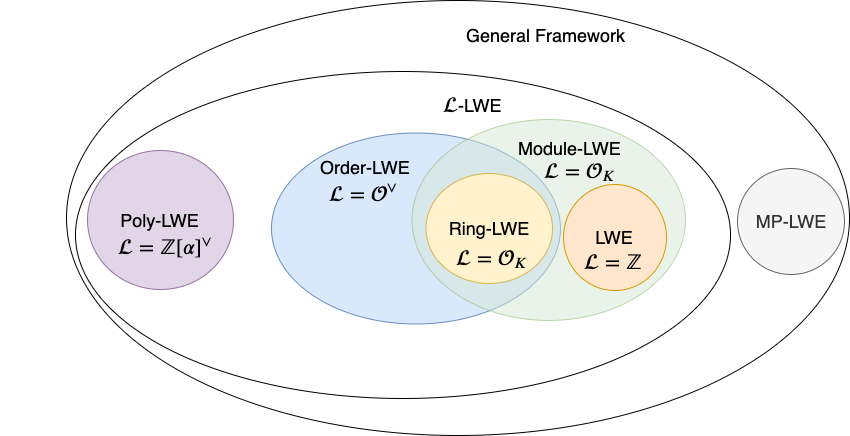
\includegraphics[width=0.45\textwidth]{files/General-LWE.png}
  	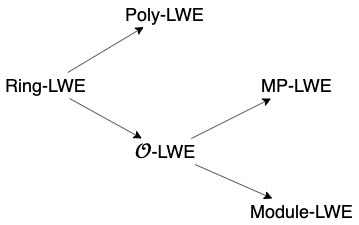
\includegraphics[width=0.45\textwidth]{files/LWE-Reductions.png}
  	\end{figure}

  \end{itemize}
}

\section{Algebraic Number Theory}
\frame
{
  \frametitle{Algebraic Number Theory}
  Let $K$ be a \blue{field extension} of $\bbQ$
  \begin{itemize}
  	\item Let degree-$d$ polynomial $f(x)\in\bbQ[X]$ \red{irreducible} over $\bbQ$
  	\item Let $\alpha\notin\bbQ$ be a \dgreen{root} of $f(x)$
  	\item $K=\bbQ(\alpha)$ is the \blue{minimal field} that contains $\alpha$
  \end{itemize}

  \noindent\rule{6cm}{0.4pt}\\
  Example:
  \begin{itemize}
  	\item $f(x)=x^2-2$ is irreducible over $\bbQ$
  	\item $\sqrt{2}\notin\bbQ$ is a root of $f(x)$
  	\item $K=\bbQ(\sqrt{2})=\{a+b\sqrt{2}\}_{a,b\in\bbQ}$
  \end{itemize}
}

\frame
{
  \frametitle{Algebraic Number Theory}
  Given a \blue{basis} $\vec{b}=(b_1,b_2,\cdots,b_d)\in K$, $K$ is isomorphic to a $d$-dimensional \dgreen{vector space} over $\bbQ$
  \begin{itemize}
  	\item $(1,\sqrt{2})$ is a basis of $\bbQ(\sqrt{2})$
  \end{itemize}

  \noindent\rule{6cm}{0.4pt}\\
  For any $x\in K$, $x$ is identified with a \blue{map} $\phi_x:K\to K$ that is \olive{multiplication by} $x$
  \begin{itemize}
  	\item $\phi_x(y)=x\cdot y$
  	\item $\phi_x$ is linear, \blue{given a basis} $\vec{b}$, $\phi_x$ is \dgreen{identified with a matrix} $M_x$
  	\item For \blue{different} basis, $M_x$ \blue{varies}, but $\Tr(M_x)$ and $\det(M_x)$ are \dgreen{invariant}
  	\item Therefore, $\TrKQ(x):=\Tr(M_x)$ and $\NKQ(x):=\det(M_x)$, called the \blue{trace} and \blue{norm} of $x$, are \dgreen{well defined}
  \end{itemize}
}

\frame
{
  \frametitle{Algebraic Number Theory}
  A \blue{lattice} $\cL\subseteq K$ is a \dgreen{discrete}, \dgreen{additive subgroup} of $K$

  \noindent\rule{6cm}{0.4pt}\\
  An \blue{order} $\cO\subseteq K$ is \blue{both} a \dgreen{lattice} and a \dgreen{subring with unity} in $K$

  \noindent\rule{6cm}{0.4pt}\\
  \begin{itemize}
  	\item The \blue{ring of integers} $\cO_K$ is the \olive{maximal order} in $K$
  	\item The \blue{coefficient ring} of $\cL$ is $\cOL:=\{x\in K:x\cL\subseteq\cL\}$ which is \dgreen{also an order} of $K$
  	\item If $\cL$ is itself an order $\cO$, then $\cOL=\cO$
  \end{itemize}
}

\frame
{
  \frametitle{Algebraic Number Theory}
  An $n$-dimensional $\cL$ \blue{lattice} admits a \dgreen{$\bbZ$-basis} $\vb=(b_1,\cdots,b_n)$ in $K$
  \begin{itemize}
  	\item The \blue{dual lattice} of $\cL$ is $\cLV:=\{x\in K:\TrKQ(x\cL)\subseteq\bbZ\}$
  	\item The \blue{dual basis} $\vbV:=(b_1^{\vee},\cdots,b_n^{\vee})$ where $\TrKQ(b_i\cdot b_j)=\delta_{ij}$ \dgreen{is a basis of} $\cLV$
  	\item $\cOL=\cO^{\cLV}$
  \end{itemize}

  \divline\\

  For $x\in\cL$, $\vb$ a basis of $\cL$, then the \blue{coordinate of $x$ under $\vb$} is $\vx=\Tr(x\cdot\vbV)$.

  \divline\\

  For $x,y\in\cL$, $\vx$ is \blue{coordinate of $x$ under $\vb$}, $\vy$ is \blue{coordinate of $y$ under $\vbV$}, then $\TrKQ(x\cdot y)=\langle\vx,\vy\rangle$
}

\frame
{
  \frametitle{Algebraic Number Theory}
  $\cL_q$ is the \blue{quotient group} $\cL/q\cL$, similarly $\cLV_q:=\cLV/q\cLV$

  \divline\\

  Field \blue{tensor product} $\KR:=K\otimes_{\bbQ}\bbR$ is the \dgreen{real analog} of $K/\bbQ$
  \begin{itemize}
  	\item If $f(x)$ has $s_1$ \blue{real roots} and $s_2$ conjugate pairs of \blue{complex roots}, then $\KR\simeq\bbR^{s_1}\times\bbC^{s_2}$
  \end{itemize}
}

\section{General Framework}
\frame
{
  \frametitle{General Framework}

  A \blue{module} of ring $\cR$ is a group $M$ operated by $\cR$ such that

  \[(a+b)x=ax+bx\qquad a(x+y)=ax+ay\qquad\forall a,b\in\cR,x,y\in M\]
  \divline\\

  \begin{itemize}
  	\item A \blue{free module} is a \blue{module} that admits a \dgreen{basis}
  	\item \blue{Free module} over rings is \orange{analogous} of \blue{vector space} over fields
  \end{itemize}
}

\frame
{
  \frametitle{General Framework}
  \textbf{Observation}: the \blue{secret} $s$, \blue{public multipliers} $a$ and \blue{product} $s\cdot a$ can be viewed as belonging to \orange{free modules} $M_s$, $M_a$ and $M_b$ over some \blue{commutative ring $\cR$} respectively.

  \divline\\

  \textbf{Multiplication}: The multiplication is \orange{generalized to} a fixed \blue{$\cR$-bilinear map} $T:M_s\times M_a\to M_b$.
  \begin{itemize}
  	\item $T$ can be represented by a \blue{order-three tensor} (like a three-dimensional matrix)
  \end{itemize}

  \divline\\

  \begin{table}[tb]
  	\centering

  	\begin{tabular}{c|ccccc}
  	\hline

  	\hline
  	\textbf{Variant} & $M_s$            & $M_a$      & $M_b$        & $T$           & \\
  	\hline
  		LWE            & $\bbZ_q^n$       & $\bbZ_q^n$ & $\bbZ_q$     & Inner product & \\
  		Ring-LWE       & $R_q^{\vee}$     & $R_q$      & $R_q^{\vee}$ & Field mult    & $R=\cO_K$ \\
  		MP-LWE         & $\bbZ_q^{n+d-1}$ & $\bbZ_q^n$ & $\bbZ_q^d$   & Hankle matrix & \\
  	\hline

  	\hline
  	\end{tabular}
  \end{table}
}

\frame
{
  \frametitle{General Framework}

  For MP-LWE, the \blue{bilinear map} $M:\bbZ_q^{n+d-1}\times\bbZ_q^n\to\bbZ_q^d$ corresponds to a $(n+d-1)\times n\times d$ tensor $M$, where the $M_{i\cdot\cdot}$'s form a \dgreen{basis of Hankle matrix}

  \begin{figure}[ht!]
  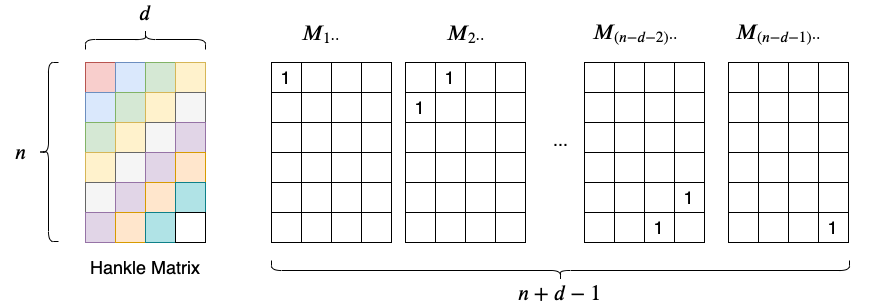
\includegraphics[width=0.8\textwidth]{files/Hankle-Matrix}
  \end{figure}

}

\section{$\cL$-LWE}
\frame
{
  \frametitle{$\cL$-LWE}
  Given $K/\bbQ$ of degree $n$
  \begin{itemize}
  	\item $\cL$ a lattice in $K$
  	\item $\cOL$ \blue{coefficient ring} of $\cL$
  	\item $\psi$ distribution over $K_{\bbR}$
  	\item $q,k$ positive integers
  	\item $\vs\in(\cLV_q)^k$ is secret vector
  \end{itemize}
  An \blue{$\cL$-LWE distribution} $A_{q,\psi}^{\cL,k}(\vs)$ over $(\cO_q^{\cL})^k\times\KR/q\cLV$ is sampled by
  \begin{itemize}
  	\item choosing \blue{uniformly} $\va\leftarrow(\cO_q^{\cL})^k$
  	\item choose $e\leftarrow\psi$
  	\item output $(a,b=\langle\vs,\va\rangle+e\bmod q\cLV)$
  \end{itemize}

}

\frame
{
  \frametitle{$\cL$-LWE}
  The \blue{decision $\cL$-LWE$_{q,\psi,\ell}^k$ problem} is to distinguish between
  \begin{itemize}
  	\item $\ell$ samples from \dgreen{$A_{q,\psi}^{\cL,k}(\vs)$ where $\vs\leftarrow U((\cLV_q)^k)$}; and
  	\item $\ell$ samples from \dgreen{uniform distribution over $(\cOL_q)^k\times\KR/q\cLV$}
  \end{itemize}

  \divline\\

  The \blue{search $\cL$-LWE$_{q,\psi,\ell}^k$ problem} is given $\ell$ samples from $A_{q,\psi}^{\cL,k}(\vs)$ for \dgreen{arbitrary $\vs\in U((\cLV_q)^k)$}, find $\vs$
}

\frame
{
  \frametitle{$\cL$-LWE}

  $\cL$-LWE generalizes the \blue{algebraic number field LWE}s.
  Variants \orange{differ in} specific choices of
  \begin{itemize}
  	\item The \blue{lattice} $\cL$
  	\item The \blue{dimension} $k$
  \end{itemize}

  \begin{table}[tb]
  	\centering

  	\begin{tabular}{c|ccccc}
  	\hline

  	\hline
  	\textbf{LWE Variants} & $\cL$ & $\cLV_q$ & $\cOL_q$ & $k$ \\
  	\hline
  		Ring-LWE & $\cR=\cO_K$ & $\cR_q^{\vee}$ & $\cR_q$ & 1 \\
  		Module-LWE & $\cR=\cO_K$ & $\cR_q^{\vee}$ & $\cR_q$ & k \\
  		Poly-LWE & $\bbZ[\alpha]^{\vee}$ & $\bbZ_q[\alpha]$ & $\bbZ_q[\alpha]$ & 1 \\
  		Order-LWE & $\cO$ & $\cO_q^{\vee}$ & $\cO_q$ & 1 \\
  	\hline

  	\hline
  	\end{tabular}
  \end{table}
}

\section{Reductions}
\frame
{
  \frametitle{Reduction from $\cL$-LWE to $\cL'$-LWE}

  \begin{block}{Lemma 4.1}
  Let $\cL'\subseteq\cL$ be lattices in number field $K$, $q$ positive integer.
  The \blue{natural inclusion map} $h:\cL_q'\to\cL_q$ is a \blue{bijection} iff $q$ is \blue{coprime} with $|\cL/\cL'|$.

  In this case, $h$ is \dgreen{efficiently computable and invertible} given arbitrary basis of $\cL'$ relatively a basis of $\cL$.
  \end{block}

  The \blue{natrual inclusion map} $\cL_q'\to\cL_q$ sends $x+q\cL'$ to $x+q\cL$.

  \divline\\

  \textbf{Proof}:
  \begin{enumerate}
  	\item Let $\vb,\vb'$ be \blue{$\bbZ$-basis} of $\cL,\cL'$, $\vb'=T\vb$, $T$ is \blue{square integral matrix}
  	\item $x'$ has coordinate $\vx'$ in $\vb'$ $\Rightarrow$ $x=h(x')$ has coordinate $\vx=T^t\vx'$ in $\vb$
  	\item $h$ is \blue{bijection} $\Leftrightarrow$ $T$ is \blue{invertible} over $\bbZ_q$ $\Leftrightarrow$ $|\det(T)|=|\cL/\cL'|$ \blue{coprime} with $q$
  \end{enumerate}
}

\frame
{
  \frametitle{Reduction from $\cL$-LWE to $\cL'$-LWE}

  \begin{block}{Lemma 4.2}
  Let $\cL'\subseteq\cL$ be lattices in number field $K$, $q$ positive integer \blue{coprime} with $|\cL/\cL'|$.
  If $\cOLp\subseteq\cO^{\cL}$ then the \blue{natural inclusion map} $g:\cOLp_q\to\cOL_q$ is a \dgreen{bijection}
  \end{block}
  \textbf{Proof}:
  \begin{enumerate}
  	\item For any $a\in\cOLp_q$, $x\in\cL_q'$, $h(a\cdot x)=g(a)\cdot h(x)$
  	\item For any $a,b\in\cOLp_q$ satisfying $g(a)=g(b)$, $h(a\cdot x)=h(b\cdot x)$
  	\item By Lemma 4.1, $h$ is bijection, so $a\cdot x=b\cdot x\bmod q\cL'$
  	\item $(a-b)\cdot\cL'\subseteq q\cL'\Rightarrow a-b\in q\cOLp\Rightarrow a=b\bmod q\cOLp$
  \end{enumerate}
}

\frame
{
  \frametitle{Reduction from $\cL$-LWE to $\cL'$-LWE}
  \begin{block}{Theorem 4.3}
  Let $\cL'\subseteq\cL$ be lattices in number field $K$, $q$ positive integer, $\psi$ distribution over $\KR$.
  If $\cOLp\subseteq\cOL$ and the \blue{natrual inclusion map} $g:\cOLp_q\to\cOL_q$ is \dgreen{efficiently invertible bijection}, there is an \orange{efficient deterministic transform}:
  \begin{enumerate}
  	\item maps \blue{uniform distribution} over $(\cOL_q)^k\times\KR/q\cLV$ to \blue{uniform distribution} over $(\cOLp_q)^k\times\KR/q\cLpV$
  	\item maps \blue{$\cL$-LWE distribution} $A_{q,\psi}^{\cL}(s)$ to \blue{$\cL'$-LWE distribution} $A_{q,\psi}^{\cL'}(s')$ where $s=s'\bmod q\cLpV$
  \end{enumerate}
  \end{block}
}

\frame
{
  \frametitle{Reduction from $\cL$-LWE to $\cL'$-LWE}
  \textbf{Proof}:
  \begin{itemize}
  	\item The transformation is: given $(a,b)\in(\cOL_q)^k\times\KR/q\cLV$, output
  	\[(a'=g^{-1}(a),b'=b\bmod q\cLpV)\]
  	\item $g$ is bijection, so $g$ sends uniform $a$ to uniform $a'$; $\cL'\subseteq\cL\Rightarrow q\cLV\subseteq q\cLpV$, so $b'$ is uniform
  	\item To show that if $b=s\cdot a+e\bmod q\cLV$ then $b'=s'\cdot a'+e\bmod q\cLpV$
  	\begin{eqnarray*}
  		a\cdot s &=& a'\cdot s + q(\cOL\cdot s) \\
  		&\subseteq& a'\cdot s + q\cLV \\
  		&\subseteq& a'\cdot(s'+q\cLpV) + q\cLV \\
  		&\subseteq& a'\cdot s'+q\cLpV
  	\end{eqnarray*}

  \end{itemize}
}

\frame
{
  \frametitle{Reduction from $\cL$-LWE to $\cL'$-LWE}
  \begin{block}{Corollary 4.4}
  Let $\cL'\subseteq\cL$ be lattices in number field $K$, $q$ positive integer \blue{coprime with $|\cL/\cL'|$}, $\psi$ distribution over $\KR$.
  If $\cOLp\subseteq\cOL$ and the bases of $\cL',\cOLp$ relative to bases of $\cL,\cOL$ are known. Then there is an \dgreen{efficient deterministic reduction} from $\cL$-LWE$_{q,\psi,\ell}$ to $\cL'$-LWE$_{q,\psi,\ell}$ for both the search and decision versions.
  \end{block}
  \textbf{Proof}:
  \begin{itemize}
  	\item By Lemma 4.1, 4.2, the \blue{natural inclusion maps} $h,g$ are efficiently \dgreen{computable and invertible bijections}
  	\item For \blue{decision problems}, use the \dgreen{transform} from Theorem 4.3 to map the input samples
  	\item For \blue{computation problems}, apply the transform and recover $s$ from $s'$ by $s=h^{-1}(s')$
  \end{itemize}
}

\frame
{
  \frametitle{Reduction from $\cO$-LWE to MP-LWE}
  \begin{block}{Definition 5.1}
  A \blue{tweaked power basis} of order $\cO$ of a number field is a $\bbZ$-basis $\vp$ of the form $t\cdot(1,x,\cdots,x^{d-1})$ for some $t,x\in\cO$
  \end{block}

  \begin{block}{Theorem 5.2}
	Let $d\leq n$ be positive integers, $\cO$ be an \blue{order} of a degree-$d$ number field $K$ \blue{with a tweaked power basis} $\vp$, $\psi$ be a \blue{distribution} over $\KR$, and $q$ a positive integer. There is an \dgreen{efficient randomized transform} which:
	\begin{enumerate}
		\item maps \blue{uniform distribution} over $\cO_q\times\KR/q\cOV$ to \blue{uniform distribution} over $\bbZ_q^n\times(\bbR/q\bbZ)^d$
		\item maps \blue{$\cO$-LWE distribution} $A_{q,\psi}^{\cO}(s)$ to \blue{MP-LWE distribution} $C_{n,d,q,\psi'}(\vs')$ where $\vs'$ is some \blue{fixed linear function} (depending only on $\vp$) of $s$, and $\psi'=\TrKRR(\psi\cdot\vp)$
	\end{enumerate}
	In particular, there is an \dgreen{efficient randomized reduction} from (search or decision) $\cO$-LWE$_{q,\psi,\ell}$ to (search or decision, respectively) MP-LWE$_{n,d,q,\psi',\ell}$.
  \end{block}
}

\frame
{
  \frametitle{Reduction from $\cO$-LWE to MP-LWE}
  \textbf{Proof}:
  \begin{itemize}
  	\item Extend $\vp$ to \blue{generating set} $\vp'$ of size $n$ by \orange{including more powers of $x$}
  	\item The transform maps $(a,b)$ to $(\va,\vb)$ where
	  	\begin{itemize}
	  		\item $\va$ is \blue{uniform random solution} to $\langle\vp',\va\rangle=a$
	  		\item $\vb$ is \blue{$\TrKRR(b\cdot\vp)$}
	  	\end{itemize}
	  \item \textbf{Uniform case}:
	  	\begin{itemize}
	  		\item The solutions to $\langle\vp',\va\rangle=0\in\cO_q$ form a subgroup $G\subseteq\bbZ_q^n$, a uniformly random $a\in\cO_q$ corresponds to a uniformly random coset of $G$
	  		\item $\TrKRR(b\cdot\vp)$ is the coordinate of $b$ under basis $\vpV$, which is an $\bbR$-basis of $\KR$
	  	\end{itemize}
	  \item \textbf{LWE case}:
	  	\begin{itemize}
	  		\item The $\cO$-LWE bilinear map $T:\cOV_q\times\cO_q\to\cOV_q$ corresponds to $(n+d-1)\times n\times d$ tensor $T_{ijk}=\TrKQ(p_i^{\vee}\cdot p_j'\cdot p_k)\bmod q$, $T_{i\cdot\cdot}$ is a $n\times d$ \blue{Hankle matrix}
	  		\item The MP-LWE bilinear map $M:\bbZ^{n+d-1}\times\bbZ^n\to\bbZ^d$ corresponds to a tensor $M_{ijk}$ where $M_{i\cdot\cdot}$'s form a basis of all Hankle matrices, so there is $(n+d-1)\times d$ matrix $P$ such that $T_{i\cdot\cdot}=\sum_{j}M_{j\cdot\cdot}P_{ji}$
	  	\end{itemize}
  \end{itemize}
}

\frame
{
  \frametitle{Reduction from $\cO$-LWE to MP-LWE}
  \textbf{Proof (Continued)}:
  \begin{itemize}
  	\item For $b=s\cdot a+e\bmod q\cOV$, let $\vs=\Tr(s\cdot\vp)\in\bbZ_q^d$, $\ve=\Tr(e,\vp)$, then $\vb=M(P\vs,\va)+\ve\bmod q\bbZ^d$
  	\item To apply the transform to get a reduction from $\cO$-LWE to MP-LWE, $\vs$ needs to be \red{rerandomized}. Choose \blue{uniformly random} $\vr\in\bbZ_q^{n+d-1}$, and \blue{replace} sample $(\va,\vb)$ with $(\va,\vb+M(\vr,\va))$
  	\item For decision problem, apply the transform directly
  	\item For search problem, recover the secret of $\cO$-LWE by $s=\langle\vpV,P_L^{-1}\vs\rangle$ where $P_L^{-1}$ is the left inverse of $P$
  \end{itemize}
}

\frame
{
  \frametitle{Reduction from $\cO$-LWE to MP-LWE}
  Theorem 5.2 transforms $\cO$-LWE with \blue{error distribution} $\psi$ to MP-LWE with \blue{error distribution} $\psi'$ which is \orange{related to $\psi$}. However, we want a reduction from \red{many} $\cO$-LWE problems to a \red{single} MP-LWE problem.
  \begin{itemize}
  	\item For $\psi$ being Gaussian distribution over $\KR$, $\psi'$ is Gaussian over $\bbR^n$
  	\item Fix some orthogonal $\bbR$-basis $\vb$ of $\KR$, let $P_b=\Tr(\vb\cdot\vp^t)$
  	\item If covariance of $\psi$ is $\Sigma$, then covariance of $\psi'$ is $\Sigma'=P_b^t\cdot\Sigma\cdot P_b$
  \end{itemize}
  \begin{block}{Corollary 5.4}
  Let $d\leq n$ be positive integers, $\cO$ be an \blue{order} of a degree-$d$ number field $K$ \blue{with a tweaked power basis} $\vp$, $\Sigma\in\bbR^{d\times d}$ a positive definite matrix, $q$ a positive integer. For any \blue{$\Sigma'\succ P_b^t\cdot\Sigma\cdot P_b$}, there is an \dgreen{efficient randomized reduction} from (search or decision) $\cO$-LWE$_{q,D_{\sqrt{\Sigma}},\ell}$ to (search or decision) MP-LWE$_{n,d,q,D_{\sqrt{\Sigma'}},\ell}$.

  In particular, for any \blue{$r'>r\cdot\|P_b\|$}, there is an \dgreen{efficient randomized reduction} from (search or decision) $\cO$-LWE$_{q,D_r,\ell}$ to (search or decision, respectively) MP-LWE$_{n,d,q,D_{r'},\ell}$.
  \end{block}
}

\frame
{
  \frametitle{Reduction from $\cO'$-LWE to $\cO$-LWE$^k$}
  \begin{block}{Theorem 6.1}
  Let $K'/K$ be a number field extension; $\cO$ be an order of $K$; $\cO'$ be an order of $K'$ that is a rank-$k$ free $\cO$-module with known basis $\vb$; $\psi'$ be a distribution over $\KR'$; and $q$ be a positive integer. There is an \dgreen{efficient deterministic transform} which:
	\begin{enumerate}
		\item maps \blue{uniform distribution} over $\cO_q'\times\KR'/q\cOpV$ to \blue{uniform distribution} over $\cO_q^k\times\KR/q\cOV$
		\item maps \blue{$\cO'$-LWE distribution} $A_{q,\psi'}^{\cO'}(s')$ to \blue{$\cO$-LWE$^k$ distribution} $A_{q,\psi}^{\cO,k}(\vs)$ for $\vs=\Tr_{K'/K}(s'\cdot\vb)\bmod q\cOV$ and $\psi=\Tr_{\KR'/\KR}(\psi')$
	\end{enumerate}
	It immediately follows that there is an \dgreen{efficient randomized reduction} from (search or decision) $\cO'$-LWE$_{q,\psi',\ell}^1$ to (search or decision, respectively) $\cO$-LWE$_{q,\psi,\ell}^k$.
  \end{block}
}

\frame
{
  \frametitle{Reduction from $\cO'$-LWE to $\cO$-LWE$^k$}
  \textbf{Proof}:
  \begin{itemize}
  	\item The transformation maps $(a',b')\in\cO_q'\times\KR'/q\cOpV$ to
  		\[(\va=\Tr(a',\vbV), b=\Tr(b')\bmod q\cOV)\in\cO_q^k\times\KR/q\cOV\]
  	\item \textbf{Uniform case}:
  		\begin{itemize}
  			\item A \dgreen{uniform} $a'$ is mapped to \dgreen{uniform} $\va$ because $\vb$ is an \blue{$\cO_q$-basis} of $\cO_q'$
  			\item A \dgreen{uniform} $b'$ is mapped to \dgreen{uniform} $b$ becase $\Tr:\KR'\to\KR$ is \blue{surjective $\KR$-linear map}, and $\Tr(\cOpV)\subseteq\cOV$
  		\end{itemize}
  	\item \textbf{LWE case}:
  		\begin{itemize}
  			\item Show that if $b'=s'\cdot a'+e'$ then $b=\langle\vs,\va\rangle+e$, for $\vs=\Tr(s',\vb)$, $e=\Tr(e')$
  			\item $s'=\langle\vs,\vbV\rangle, a'=\langle\va,\vb\rangle\Rightarrow\Tr(s'\cdot a')=\langle\vs,\va\rangle$
  		\end{itemize}
  	\item \textbf{Reductions}:
  		\begin{itemize}
  			\item Decision problem: directly apply the above transform
  			\item Search problem: recover $s$ from $\vs$ by $s=\langle\vs,\vbV\rangle$
  		\end{itemize}
  \end{itemize}
}

\frame
{
  \frametitle{Reduction from $\cO'$-LWE to $\cO$-LWE$^k$}
  Similar to Theorem 5.1, $\psi'$ is \orange{related to} $\psi$, so our reduction is \red{one-to-one}. To obtain \dgreen{many-to-one} reduction, consider the case where \blue{$\psi'$ is Gaussian}
  \begin{itemize}
  	\item Fix orthonormal $\bbR$-bases $\vc$, $\vc'$ of $\KR,\KR'$ respectively, let matrix $A=\TrKRpR(\vc'\cdot(\vcV)^t)$,
  	\item If $\psi'$ is Gaussian with covariance $\Sigma'$ under $\vc'$, then $\psi$ is Gaussian with covariance $\Sigma_1=A^t\cdot\Sigma'\cdot A$ under $\vc$
  \end{itemize}
  \begin{block}{Corollary 6.2}
  Adopt the notation and hypothesis of Theorem 6.1, with $\psi'=D_{\Sigma'}$ over $\KR'$ for some positive definite matrix $\Sigma'$. For any $\Sigma\succ A^t\cdot\Sigma'\cdot A$, there is an \dgreen{efficient, randomized} reduction from (search or decision) $\cO'$-LWE$_{q,D_{\Sigma'},\ell}^1$ to (search or decision) $\cO$-LWE$_{q,D_{\Sigma},\ell}^k$.

  Moreover, for $r=r'\sqrt{k}$, there is an \dgreen{efficient deterministic reduction} from (search or decision) $\cO'$-LWE$_{q,D_{r'},\ell}^1$ to (search or decision, respectively) $\cO$-LWE$_{q,D_{r},\ell}^k$.
  \end{block}
}

\frame
{
	\Huge\center Thank you
}

\end{document}
